\documentclass{beamer}
\usetheme{Boadilla}

\makeatother
\setbeamertemplate{footline}
{
    \leavevmode%
    \hbox{%
    \begin{beamercolorbox}[wd=.4\paperwidth,ht=2.25ex,dp=1ex,center]{author in head/foot}%
        \usebeamerfont{author in head/foot}\insertshortauthor
    \end{beamercolorbox}%
    \begin{beamercolorbox}[wd=.55\paperwidth,ht=2.25ex,dp=1ex,center]{title in head/foot}%
        \usebeamerfont{title in head/foot}\insertshorttitle
    \end{beamercolorbox}%
    \begin{beamercolorbox}[wd=.05\paperwidth,ht=2.25ex,dp=1ex,center]{date in head/foot}%
        \insertframenumber{}
    \end{beamercolorbox}}%
    \vskip0pt%
}
\makeatletter
\setbeamertemplate{navigation symbols}{}

\usepackage[T1]{fontenc}
\usepackage{lmodern}
\usepackage{amssymb,amsmath}
\renewcommand{\familydefault}{\sfdefault}

\DeclareMathOperator*{\argmax}{argmax}

\usepackage{mathtools}
\usepackage{graphicx}
\usepackage{threeparttable}
\usepackage{booktabs}
\usepackage{siunitx}
\sisetup{parse-numbers=false}

%\setlength{\OuterFrameSep}{-2pt}
%\makeatletter
%\preto{\@verbatim}{\topsep=-10pt \partopsep=-10pt }
%\makeatother

\title[Lecture 6:\ Maximum Likelihood Estimation]{Lecture 6:\ Maximum Likelihood Estimation}
\author[ResEcon 703:\ Advanced Econometrics]{ResEcon 703:\ Topics in Advanced Econometrics}
\date{Matt Woerman\\University of Massachusetts Amherst}

\begin{document}

{\setbeamertemplate{footline}{} 
\begin{frame}[noframenumbering]
    \titlepage
\end{frame}
}

\begin{frame}\frametitle{Agenda}
    Last time
    \begin{itemize}
        \item Logit Model
    \end{itemize}
    \vspace{2ex}
    Today
    \begin{itemize}
    	\item Nonlinear Regression Models
        \item Maximum Likelihood Estimation
        \item Properties of the Maximum Likelihood Estimator
    \end{itemize}
    \vspace{2ex}
    Upcoming
    \begin{itemize}
        \item Reading for next time
        \begin{itemize}
            \item Train textbook, Chapter 8
        \end{itemize}
        \item Problem set
        \begin{itemize}
            \item Problem Set 1 is posted, due September 24
        \end{itemize}
    \end{itemize}
\end{frame}

\begin{frame}\frametitle{Recap and Looking Ahead}
    So far
    \begin{itemize}
        \item Discrete choice framework
        \item Random utility model
        \item Logit model
    \end{itemize}
    \vspace{3ex}
    But we still do not know how to estimate the logit model! \\
    \vspace{3ex}
    Coming up
    \begin{itemize}
        \item Maximum likelihood estimation
        \item Numerical optimization
        \item Estimating the logit model
    \end{itemize}
\end{frame}

\begin{frame}\frametitle{}
    \vfill
    \centering
    \begin{beamercolorbox}[center]{title}
        \Large Nonlinear Regression Models
    \end{beamercolorbox}
    \vfill
\end{frame}

\begin{frame}\frametitle{Nonlinear Regression Models}
    The general formula for a nonlinear regression model
    $$y_i = h(x_i, \theta) + \varepsilon_i$$
    \begin{itemize}
        \item OLS (linear model) is a special case
        \item Some models that appear to be nonlinear can be simplified to a linear model
        \begin{itemize}
            \item See the Cobb-Douglas production function example from Lecture 1
        \end{itemize}
    \end{itemize}
\end{frame}

\begin{frame}\frametitle{Examples of Nonlinear Regression Models}
    Binary discrete choice
    \begin{align*}
        u_i &= \beta' x_i + \varepsilon_i \\
        y_i &= 
            \begin{cases}
                1 & \text{ if } u_i > 0 \\
                0 & \text{ otherwise}
            \end{cases}
    \end{align*}
    \vspace{1ex}
    CES production function
    $$\ln y_i = \ln \gamma - \frac{\upsilon}{\rho} \ln \left[ \delta K_i^{-\rho} + \left( 1 - \delta \right) L_i^{-\rho} \right] + \varepsilon_i$$
    \vspace{1ex}
    Exponential regression
    $$y_i = \beta_0 + \beta_1 e^{\beta _2 x_{i1} + \beta_3 x_{i2}} + \varepsilon _i$$
\end{frame}

\begin{frame}\frametitle{Nonlinear Regression Assumptions}
    \textbf{Assumption 1: Functional form} \\
    \vspace{3ex}
    The conditional mean function of observation $y_i$ given $x_i$ is
    $$E(y_i \mid x_i) = h(x_i, \theta)$$
    where $h(x_i, \theta)$ is a continuously differetiable function of $\theta$
\end{frame}

\begin{frame}\frametitle{Nonlinear Regression Assumptions}
    \textbf{Assumption 2: Identifiability of the model parameters} \\
    \vspace{3ex}
    The parameter vector in the model is identified (estimable) if there is no nonzero parameter $\theta^0 \neq \theta$ such that $h(x_i, \theta^0) = h(x_i, \theta)$ for all $x_i$
    \begin{itemize}
         \item There cannot be a second set of parameters, $\theta^0$, that gives the exact same model fit as the true parameters, $\theta$
         \begin{itemize}
             \item The logit model is not identified without normalizing the scale parameter (setting $\sigma = 1$) because we could multiply the coefficients and scale parameter by the same constant to get a $\beta^0$ and $\sigma^0$ that fit the model exactly the same
         \end{itemize}
         \item In the linear model, this was the full rank assumption, but the simple absence of ``multicollinearity'' among the variables in $x_i$ is not sufficient to produce this condition in the nonlinear regression model
     \end{itemize} 
\end{frame}

\begin{frame}\frametitle{Nonlinear Regression Assumptions}
    \textbf{Assumption 3: Zero mean of the disturbance} \\
    \vspace{3ex}
    It follows from Assumption 1 that we may write
    $$y_i = h(x_i, \theta) + \varepsilon_i$$
    where 
    $$E[\varepsilon_i \mid h(x_i, \theta)] = 0$$ \\
    \begin{itemize}
        \item The error at observation $i$ is uncorrelated with the conditional mean function, which is not necessarily the same as assuming that the errors and the exogenous variables are uncorrelated
        \item In the linear model, the conditioning argument of this assumption is the independent variables $x_i$, but here the entire conditional mean function $h(x_i, \theta)$ is the conditioning argument
    \end{itemize}
\end{frame}

\begin{frame}\frametitle{Nonlinear Regression Assumptions}
    \textbf{Assumption 4: Homoskedasticity and nonautocorrelation} \\
    \vspace{3ex}
    As in the linear model, we assume conditional homoskedasticity
    $$E[\varepsilon_i^2 \mid h(x_j, \theta) \; \forall j] = \sigma^2 \text{ (a finite constant)}$$
    and nonautocorrelation
    $$E[\varepsilon_i \varepsilon_j \mid h(x_k, \theta) \; \forall k] = 0 \; \forall j \neq i$$ \\
    \begin{itemize}
        \item In the linear model, the conditioning argument of this assumption is the full set of independent variables, $X$
    \end{itemize}
\end{frame}

\begin{frame}\frametitle{Nonlinear Regression Assumptions}
    \textbf{Assumption 5: Data generating process} \\
    \vspace{3ex}
    The data generating process for $x_i$ is assumed to be a well-behaved population such that first and second moments of the data can be assumed to converge to fixed, finite population counterparts
    \begin{itemize}
        \item The process generating $x_i$ is strictly exogenous to that generating $\varepsilon_i$
        \item The data on $x_i$ are assumed to be ``well behaved''
    \end{itemize}
\end{frame}

\begin{frame}\frametitle{Nonlinear Regression Assumptions}
    \textbf{Assumption 6: Underlying probability model} \\
    \vspace{3ex}
    There is a well-defined probability distribution generating $\varepsilon _i$. At this point, we assume only that this process produces a sample of uncorrelated, identically (marginally) distributed random variables $\varepsilon_i$ with mean zero and variance $\sigma^2$ conditioned on $h(x_i, \theta)$.
    \begin{itemize}
        \item This assumption implies our general model is semiparametric
        \item We will soon impose additional assumptions for our structural estimation methods
    \end{itemize}
\end{frame}

\begin{frame}\frametitle{Estimating a Nonlinear Regression Model}
    Once we specify a nonlinear regression model, we have a few ways to estimate its parameters
    \begin{itemize}
        \item Maximum likelihood estimation (MLE)
        \item Nonlinear least squares (NLS)
        \item Generalized method of moments (GMM)
    \end{itemize}
    \vspace{3ex}
    MLE and NLS will impose additional assumptions on $\varepsilon_i$, but GMM is free from additional assumptions
\end{frame}

\begin{frame}\frametitle{}
    \vfill
    \centering
    \begin{beamercolorbox}[center]{title}
        \Large Maximum Likelihood Estimation
    \end{beamercolorbox}
    \vfill
\end{frame}

\begin{frame}\frametitle{Maximum Likelihood Estimation Assumption}
    \textbf{MLE Assumption} \\
    \vspace{3ex}
    The probability density function (PDF) for a random variable, $y$, conditioned on a set of parameters, $\theta$, is
    $$f(y \mid \theta)$$ \\
    \begin{itemize}
        \item This function identifies the data generating process that underlies an observed sample of data and provides a mathematical description of the data that the process will produce
        \item We are making an assumption about the density of $y$, not just its expectation and variance
    \end{itemize}
\end{frame}

\begin{frame}\frametitle{Likelihood Function}
    The joint density of $n$ independent and identically distributed (i.i.d.) from this process is
    \begin{align*}
        f(y_1, \ldots, y_n \mid \theta) &= \prod_{i = 1}^n f(y_i \mid \theta) \\
        \intertext{We switch the conditioning and define the likelihood function as a function of the unknown parameters, $\theta$, conditioned on the data we observe, $y$}
        L(\theta \mid y) &= \prod_{i = 1}^n f(y_i \mid \theta) \\
        \intertext{It will usually be easier to work with the log of the likelihood function, which is called the log-likelihood function}
        \ln L(\theta \mid y) &= \sum_{i = 1}^n \ln f(y_i \mid \theta)
    \end{align*}
\end{frame}

\begin{frame}\frametitle{Maximum Likelihood Estimator}
    The maximum likelihood estimator is the estimator that maximizes the likelihood function
    \begin{align*}
        \hat{\theta} &= \argmax_\theta L(\theta \mid y) \\
        \intertext{Because natural log is a montonic function, the estimator also maximizes the log-likelihood function}
        \hat{\theta} &= \argmax_\theta \ln L(\theta \mid y)
    \end{align*}
    A necessary condition for maximizing $\ln L(\theta \mid y)$ is
    $$\frac{\partial \ln L(\theta \mid y)}{\partial \theta} = 0$$
    This estimator gives the parameter value(s) that maximizes the likelihood of having observed the data that we did observe
\end{frame}

\begin{frame}\frametitle{Graphical Example of Maximum Likelihood}
    We have some data from a Poisson distribution. What is the $\lambda$ parameter of that distribution?
    \begin{align*}
        L(\lambda \mid y) &= \frac{e^{-n \lambda} \lambda^{\sum_{i=1}^n y_i}}{\prod_{i = 1}^n y_i!} \\
        \ln L(\lambda \mid y) &= -n \lambda + \ln \lambda \sum_{i = 1}^n y_i - \sum_{i = 1}^n \ln (y_i!)
    \end{align*}
    \begin{center}
        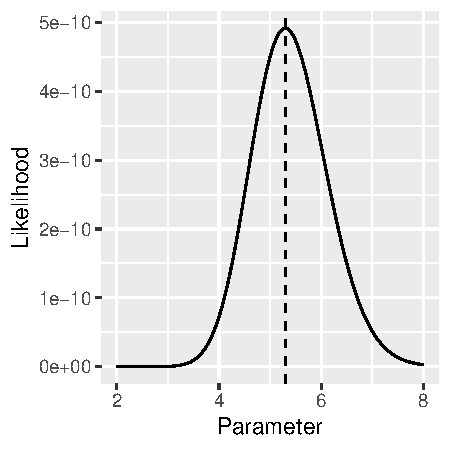
\includegraphics[width=0.4\textwidth]{likelihood.pdf}
        \hspace{5ex}
        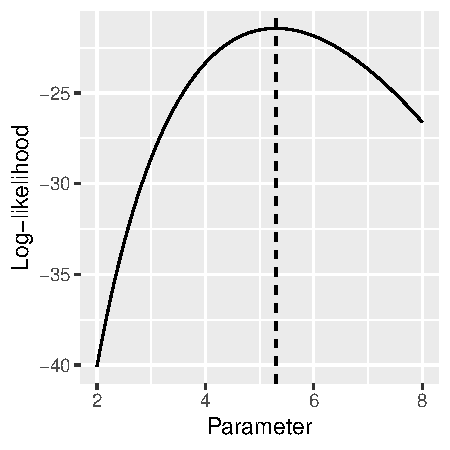
\includegraphics[width=0.4\textwidth]{log_likelihood.pdf}
    \end{center}
\end{frame}

\begin{frame}\frametitle{Conditional Likelihood}
    So far, we have assume $y$ is function of parameters, but we also want to allow it to be a function of (or conditional on) exogenous variables, $x$
    $$f(y \mid x, \alpha)$$
    Then we can write the conditional log-likelihood function as
    \begin{align*}
        \ln L(\alpha \mid x, y) = \sum_{i = 1}^n \ln f(y_i \mid x_i, \alpha) + \sum_{i = 1}^n \ln g(x_i \mid \alpha) \\
        \intertext{If these densities depend on mutually exclusive sets of parameters; that is, if we can partition $\alpha$ into $[\theta, \delta]$ and write}
        \ln L(\theta, \delta \mid x, y) = \sum_{i = 1}^n \ln f(y_i \mid x_i, \theta) + \sum_{i = 1}^n \ln g(x_i \mid \delta)
    \end{align*}
    then the conditional likelihood can almost always be treated as likelihood and the the ``conditional'' is dropped for convenience
\end{frame}

\begin{frame}\frametitle{}
    \vfill
    \centering
    \begin{beamercolorbox}[center]{title}
        \Large Properties of the Maximum Likelihood Estimator
    \end{beamercolorbox}
    \vfill
\end{frame}

\begin{frame}\frametitle{Asymptotic Properties of MLE}
    Under certain regularity conditions (we will get to these at the end), the maximum likelihood estimator (MLE) has these properties
    \begin{enumerate}
        \item Consistency
        \item Asymptotic normality
        \item Asymptotic efficiency
        \item Invariance
    \end{enumerate}
\end{frame}

\begin{frame}\frametitle{Consistency of MLE}
    The MLE, $\hat{\theta}$, converges in probability to the true parameter value(s), $\theta_0$
    $$\hat{\theta}\overset{p}{\rightarrow} \theta_0$$ \\
    \begin{itemize}
        \item As our sample size grows (to infinity), the MLE becomes vanishingly close to the true parameter value(s)
    \end{itemize}
\end{frame}

\begin{frame}\frametitle{Asymptotic Normality of MLE}
    The asymptotic distribution of the MLE, $\hat{\theta}$, is normal with mean at the true parameter value(s), $\theta_0$, and known variance
    $$\hat{\theta} \overset{a}{\sim} N(\theta_0, I(\theta_0)^{-1})$$
    where
    $$I(\theta_0) = -E_0 \left[ \frac{\partial^2 \ln L(\theta_0)}{\partial \theta_0 \partial \theta_0'} \right]$$
    \begin{itemize}
        \item The asymptotic variance (or variance-covariance matrix) of the MLE
        $$Var(\hat{\theta}) = \left\{ -E_0 \left[ \frac{\partial^2 \ln L(\theta_0)}{\partial \theta_0 \partial \theta_0'} \right] \right\}^{-1}$$
        \item We are more certain of the MLE when the likelihood function has more curvature
    \end{itemize}
\end{frame}

\begin{frame}\frametitle{Asymptotic Efficiency of MLE}
    The MLE, $\hat{\theta}$, is asymptotically efficient and achieves the Cram\'er-Rao lower bound
    $$Var(\hat{\theta}) = I(\theta_0)^{-1}$$
    \begin{itemize}
        \item No consistent estimator has lower asymptotic mean sqaured error than the MLE
    \end{itemize}
\end{frame}

\begin{frame}\frametitle{Invariance of MLE}
    The MLE of $\gamma_0 = c(\theta_0)$ is $c(\hat{\theta})$ if $c(\theta_0)$ is continuous and continuously differentiable, where $\hat{\theta}$ is the MLE of true parameter(s) $\theta_0$
    \begin{itemize}
        \item The MLE of a function of some parameter(s) is the function applied to the MLE of the parameter(s)
    \end{itemize}
\end{frame}

\begin{frame}\frametitle{Regularity Conditions for MLE}
    The preceding properties are true only if the following regularity conditions are met
    \begin{enumerate}
        \item The first three derivatives of $\ln f(y_i \mid \theta)$ with respect to $\theta$ are continuous and finite for almost all $y_i$ and for all $\theta$. This condition ensures the existence of a certain Taylor series approximation to and the finite variance of the derivatives of $\ln L(\theta)$.
        \item The conditions necessary to obtain the expectations of the first and second derivatives of $\ln f(y_i \mid \theta)$ are met.
        \item For all values of $\theta$, $\left\vert \frac{\partial^3 \ln f(y_i \mid \theta)}{\partial \theta_j \partial \theta_k \partial \theta_l} \right\vert$ is less than a function that has a
        finite expectation. This condition will allow us to truncate the Taylor series.
    \end{enumerate}
\end{frame}

\begin{frame}\frametitle{MLE Variance Estimator}
    From the asymptotic normality of MLE, we have
    $$Var(\hat{\theta}) = \left\{ -E_0 \left[ \frac{\partial^2 \ln L(\theta_0)}{\partial \theta_0 \partial \theta_0'} \right] \right\}^{-1}$$
    \begin{itemize}
        \item Variance of the MLE is evaluated at $\theta_0$, the true parameter value(s)
        \item But we do not know the true value(s), so we also need an estimator for the variance of the MLE
    \end{itemize}
    \vspace{2ex}
    We can estimate this variance by evaluating it at the MLE, $\hat{\theta}$
    $$\widehat{Var}(\hat{\theta}) = \left\{ - \left[ \frac{\partial^2 \ln L(\theta)}{\partial \theta \partial \theta'} \right]_{\hat{\theta}} \right\}^{-1}$$
    \begin{itemize}
        \item The innermost term is the Hessian of the log-likelihood function
        \item More robust estimators exist, but we will stick with this most basic variance estimator for now
    \end{itemize}
\end{frame}

\begin{frame}\frametitle{Value of Likelihood Function}
    The likelihood function evaluated at the MLE, $L(\hat{\theta})$, gives us some idea of how well our model fits the data, especially when compared to the likelihood function evaluated at some other parameter values \\
    \vspace{3ex}
    We can use these comparisons to 
    \begin{itemize}
        \item Say something about a model's goodness of fit
        \item Conduct hypothesis tests
    \end{itemize}
\end{frame}

\begin{frame}\frametitle{Likelihood Ratio Index}
    One measure of how well a MLE fits the data is the likelihood ratio index
    $$\rho = 1 - \frac{\ln L(\hat{\theta})}{\ln L(0)}$$
    where $L(0)$ measures the fit of a model with only a constant term (all other parameters equal to 0)
    \begin{itemize}
        \item This index looks like $R^2$ and is sometimes called a ``pseudo $R^2$''
        \item But this name is misleading because this metric is nothing like $R^2$ other than having the same range of $[0, 1]$
    \end{itemize}
    \vspace{2ex}
    Larger values of $\rho$ imply a better model fit, but this is no different from saying larger values of the likelihood function are better
\end{frame}

\begin{frame}\frametitle{Likelihood Ratio Test}
    The likelihood ratio test is used to test hypotheses about parameters
    $$H_0 \text{: Some restriction on the parameters } \theta$$
    We estimate the model with and without the restrictions, yielding
    \begin{itemize}
        \item $\hat{\theta}_U$: Unrestricted MLE
        \item $\hat{\theta}_R$: Restricted MLE
    \end{itemize}
    \vspace{2ex}
    The likelihood ratio is
    $$\lambda = \frac{L(\hat{\theta}_R)}{L(\hat{\theta}_U)}$$
    which has the range $(0, 1)$ and is distributed
    $$\lambda \sim \chi^2(r)$$
    where $r$ is the number of restrictions
\end{frame}

\begin{frame}\frametitle{Announcements}
    Reading for next time
    \begin{itemize}
        \item Train textbook, Chapter 8
    \end{itemize}
    \vspace{3ex}
    Upcoming
    \begin{itemize}
        \item Problem Set 1 is posted, due September 24
    \end{itemize}
\end{frame}

\end{document}